\documentclass[tikz,fontsize=8pt]{standalone}
\usepackage{fourier}
\usetikzlibrary{arrows.meta}
\usetikzlibrary{calc}
\tikzset{>=latex}
\definecolor{bookblue}{RGB}{0,173,239}
\definecolor{bookpink}{RGB}{236,0,140}
\definecolor{bookgreen}{RGB}{50,200,0}
\definecolor{bookbluearea}{RGB}{204,239,252}
\tikzstyle{blueline}=[draw=bookblue,line width=0.2mm]
\tikzstyle{pinkline}=[draw=bookpink,line width=0.2mm]
\tikzstyle{greenline}=[draw=bookgreen,line width=0.2mm]
\tikzstyle{blackline}=[draw=black,line width=0.2mm]
\tikzstyle{bluearea}=[fill=bookbluearea]

\usepackage{scrextend}
\usepackage{ifthen}
\changefontsizes[8pt]{8pt}
\usetikzlibrary{decorations.pathreplacing}
\begin{document}
  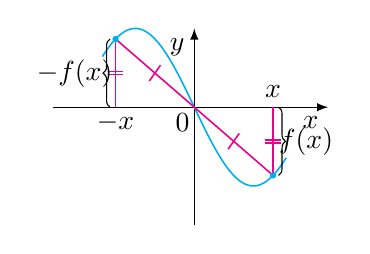
\begin{tikzpicture}
  \node at (-0.15,-0.2) {0};
  \draw[->] (-1.8,0) -- (1.7,0) node[below left] {$x$};
  \draw[->] (0,-1.5) -- (0,1) node[below left] {$y$};
  
  \draw[blueline,domain=-140:140,samples=500] plot [smooth] (\x/120,{-sin(\x)});
  \foreach \x in {0,...,1}{
    \xdef\angle{120};
    \pgfmathsetmacro\xcoord{((\x*2-1)*\angle)/120};
    \pgfmathsetmacro\ycoord{-sin((\x*2-1)*\angle)};
    %\xdef\xlabel{\ifthenelse{\xcoord>0}{x}{-x}};
    \draw[bookpink,line width=0.2mm](\xcoord,0) -- (\xcoord,\ycoord);
    \draw[bookpink,line width=0.2mm](0,0) -- (\xcoord,\ycoord);
    \draw[bookpink,line width=0.2mm]({\xcoord/2-0.0707},{\ycoord/2-0.1}) -- ({\xcoord/2+0.0707},{\ycoord/2+0.1});
    \draw[bookpink,line width=0.2mm]({\xcoord-0.1},{\ycoord/2-0.02}) -- ({\xcoord+0.1},{\ycoord/2-0.02});
    \draw[bookpink,line width=0.2mm]({\xcoord-0.1},{\ycoord/2+0.02}) -- ({\xcoord+0.1},{\ycoord/2+0.02});
    \fill[bookblue] (\xcoord,\ycoord) circle (0.4mm);
    \pgfmathsetmacro\signal{\xcoord < 0 ? "-" : ""};
    \pgfmathsetmacro\mirrorring{\xcoord < 0 ? int(1):int(0)};
    
    \ifthenelse{\mirrorring=1}{
      \node at (\xcoord, -0.2) {$\signal x$};
      \draw [decorate,decoration={brace},xshift=-2pt,yshift=0pt]
      (\xcoord,0) -- (\xcoord,\ycoord) node [midway,xshift=-0.45cm] 
      {$\signal f(x)$};
    }{
      \node at (\xcoord, 0.2) {$\signal x$};
      \draw [decorate,decoration={brace},xshift=2pt,yshift=0pt]
      (\xcoord,0) -- (\xcoord,\ycoord) node [midway,xshift=0.35cm] 
      {$\signal f(x)$};
    }
    %\fill[bookpink] ({\st*(\qtd - \qtd/\x)},0) circle (0.6mm);
  }
  %\node at (0.5,-0.25) {$1$};
  %\node at (-0.15,0.5) {$1$};
  %\draw (0.5,-0.08) -- (0.5,0.08);
  %\draw (-0.08,0.5) -- (0.08,0.5);
  %\node at (1.3,2) {$(2,4)$};
  %\node at (1.2,1) {$y=x^2$};
  %\node at (-0.9,0.5) {$(-1,1)$};
  \end{tikzpicture}
\end{document}